\documentclass[12pt,fleqn]{article}\usepackage{../common}
\begin{document}
Lineer Cebir - Ders 1

Ilk dersimize hosgeldiniz, ben Gilbert Strang. Lineer cebirin cozmeye
calistigi en temel problem bir lineer denklem sistemini cozmektir. Bu
baglamda mesela en genel durum ``bilinmeyen ve denklem sayisinin birbirine
esit oldugu'' durumdur, ki bu ``guzel durum'' olarak nitelenebilir. 

Devam edersek, dersin kavramlarini anlamak icin ``satir bakisi''na
basvuracagiz, bu durumda her denkleme teker teker bakiyoruz gibi olacak,
dersimizde pek cok kez kullanacagimiz $A$ matrisimiz olacak mesela, ve bu
matrisin satirlarin her denklemin degiskenlerinin katsayilarina tekabul
edecek.

Kolon bakis acisi belki daha once gormediginiz bir aci olacak, bu durumda
her kolon ayri ayri islenecek. 

Cebirsel bakis acisi ise tum matrisi, bu durumda $A$, ayni anda ele alir. 

Guzel durumdan baslayalim; iki bilinmeyen, iki denklem.

$$ 2x - y = 0 $$

$$ -x + 2y = 3 $$

Katsayilari matrise tasiyalim

$$ 
\left[\begin{array}{cc}
2 & -1 \\
-1 & 2
\end{array}\right]
\left[\begin{array}{c}
x \\
y
\end{array}\right]
=
\left[\begin{array}{c}
0 \\
3
\end{array}\right]
 $$

Soldaki matrise ben cogunlukla $A$ derim, sonra icinde bilinmeynleri
tasiyan $x$ vektoru koyarim, ki bazilari bunu vektor oldugu icin koyu
renkte $\mathbf{x}$ olarak ta yazar, ve sonra bir vektor daha, ki buna ben
cogunlukla $b$ derim, yani sonuc soyle olur,

$$ A x = b $$

Simdi satir bakisina basvuralim. Grafik olarak dusunelim, hangi noktalar
$2x - y = 0$ denklemini tatmin eder? Orijin $(0,0)$ noktasi bunlardan biri,
ya da $x=1,y=2$. 

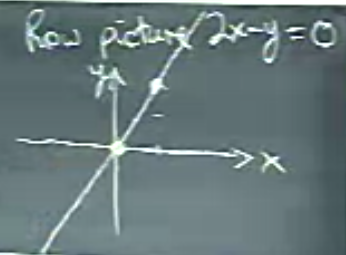
\includegraphics[height=4cm]{1_01.png}








\end{document}
